\documentclass{article}
\usepackage{graphicx} % Required for inserting images
\usepackage{cite}
\usepackage{setspace}
\usepackage{verbatimbox}

\title{NHL Meter}
\author{Alexander Hagood \& Alexander Barran}
\date{November 2024}
\doublespacing
\begin{document}

\maketitle

\section{Abstract}
The objective of this project is to provide a system that can provide live estimations
about the outcomes of a National Hockey League (NHL) game. Using statistical and
machine learning methods, we were able to create a model that can ???
\section{Introduction}
Inspired by visualizations like the Win Probability graph provided by ESPN, we sought
out to create a similar metric based on Hockey play by play data sourced from the NHL.
We would like to use information about the state of the game, such as the current 
score, 'momentum,' and other factors that can be derived from the data to determine 
the odds of the home team winning at any arbitrary point in the game. Sports are 
inherently unpredictable, however we can still make educated guesses at the chances 
of specific outcomes based on information we have. Our approach is to stream in ‘Play-By-Play’ 
data representing certain game events into our model, and then use statistical and machine 
learning techniques like logistic regresion and machine learning to update our estimation on who
is more likely to win as we gain more information about the state of the game.


\section{Problem Definition}
Given the Play-By-Play data for a specific NHL match up to a certain time point, 
what is the probability of the Home or Away team winning? With the rise of the sports 
betting industry, these types of endeavors have grown in popularity and interest on 
both the bettor and bookkeepers sides, as bettors seek new edges and bookkeepers seek 
to set more accurate lines. Estimations of NHL outcomes are not new, but from our research 
there is no investigation into the dynamic estimation as the game is played. Measuring
this probability can give us insight into the nature the moment an underdog team might
turn the tables on a strong team, or show how a dominant team can maintain control of the game.


\section{Models, Algorithms and Measures}

In order to measure the comparative strength of two teams, it is not neccesary to reinvent the wheel. 
Elo is a metric that lets us quantify this strength in a of teams, derived from the results of previous head to head match ups.
Upon completing a game, you receive Elo score corresponding to the difference between your score and your opponents. Win a game against
an opponent with a much higher score, and you receive more points than winning one with a lower score, and vice versa for losing.
Once you have these scores, you can measure the probability of a given team winning against another in a match up. 
Using the following formula we can determien the probability of a given Elo matchup resulting in a win.
\[E_{A} = \frac{1}{1 + 10^{(R_{B} - R_{A})/400}}\] 


\section{Implementation and Analysis}
Our data is sourced from the official NHL API. This allows you to get historical play-by-play 
data from games since the 2007 season using HTTP requests. Using a Game ID, you can download 
all the games for a specific season. Thankfully, there exists an existing python implementation 
that scrapes this data. 'hockey-scraper' by harryshomer on pypi allows you to input a season
or a date range, and will download the season information then all associated plays with
each game in that season. This is a somewhat large amount of data, taking multiple days to 
download due to API rate limiting. Post-parquet compression, the data including play-by-play
and shifts (documenting when a player comes on or off the ice) took up approximately half a gigabyte.

Analyzing the format of the data, we can view useful information about the game. A "play" is 
recorded whenever a notable event occurs. These events can take forms like a shot on goal, 
a successful goal, the result of a face off, penalties, or other associated game events. 
For every play, all players that were involved are listed, as well as all other players on 
the ice at the time. Spatial data is included, such as the X and Y coordinates on the rink 
where the event happened, and of course information about the game itself such as the current 
score, the teams, and the time remaining in the period.

In order to start adjusting the probability of a given team winning, you need a beginning assumption.
You could just assume that each time has an equal chance of winning, but this naive assumption 
neglects variables such as the strength of a team. We use the Elo system to determine this assumption. Starting in the 2007 season, we gave each team a 
base level of 1500 Elo, and then started feeding in the results of their match ups. Teams do maintain some level
of continuity between seasons, so instead of starting from scratch we simply shifted their Elo scores towards the baseline, 
instead of completing reseting them. When it comes time to analyze the a specific game, we can now feed in this Elo score to get a baseline expectation of win probability.

Using our Elo score at the beginning of a game, we can, we can start to adjust it based on game events. First, we subdivide the
game into discrete time slices of 30 seconds. We can then recrord the events of importance that occur during those time slices
such as goals or penalties. Using these events we can update a 'strength' score for the team. This strength score can help predict how
likely a team is to score in the near future. 

Testing our model is not as simple as one might think, as there is clearly no objective answer representing the true probability of a team winning given
a given set of circumstances that we can compare our results to. However, we can measure how accurately our model can predict probabilties in aggregate by 'backtesting' it.
There are two different methodologies we came up with to backtest our model. 

The first type we came up with is through using statistical regression methods. 
First, we group together games or plays with similar expected outcomes, such as all games around 70\% home team win probability. We can then see measure how often
the home team won in this set of games, and compare it to our model's prediction. We repeat this for all probability 'buckets' which can be at any arbitrary precision.
Once we have the True win rate, and the expected win rate, we can perform statistical methods to such as sum of least squares or logistic loss. These functions measure 'Goodness of Fit,' 
or generally represent how accurate our model is. 

There exists other types of backtesting that we can apply that are called 'scoring rules.' These are evaluation metrics that can be used to evaluate the accuracy of probabilistic predictions.
These types of scoring rules are highly applicable to our project, as we are directly making these types of forecasts and would like to measure their accuracy. By using these rules we can attempt to
minimize our distance from true probability. The scoring function we used is called Ranked Probability Score. 


\begin{minipage}{0.45\textwidth}
  \vspace*{0pt}
  \centering
  \begin{verbatim}
    Sum of Least Squares: 12.2505
    Cross Entropy: 0.8863
    Ranked Probability Score: 0.1228
  \end{verbatim}
  \end{minipage}
  \hfill
  \begin{minipage}{0.45\textwidth}
  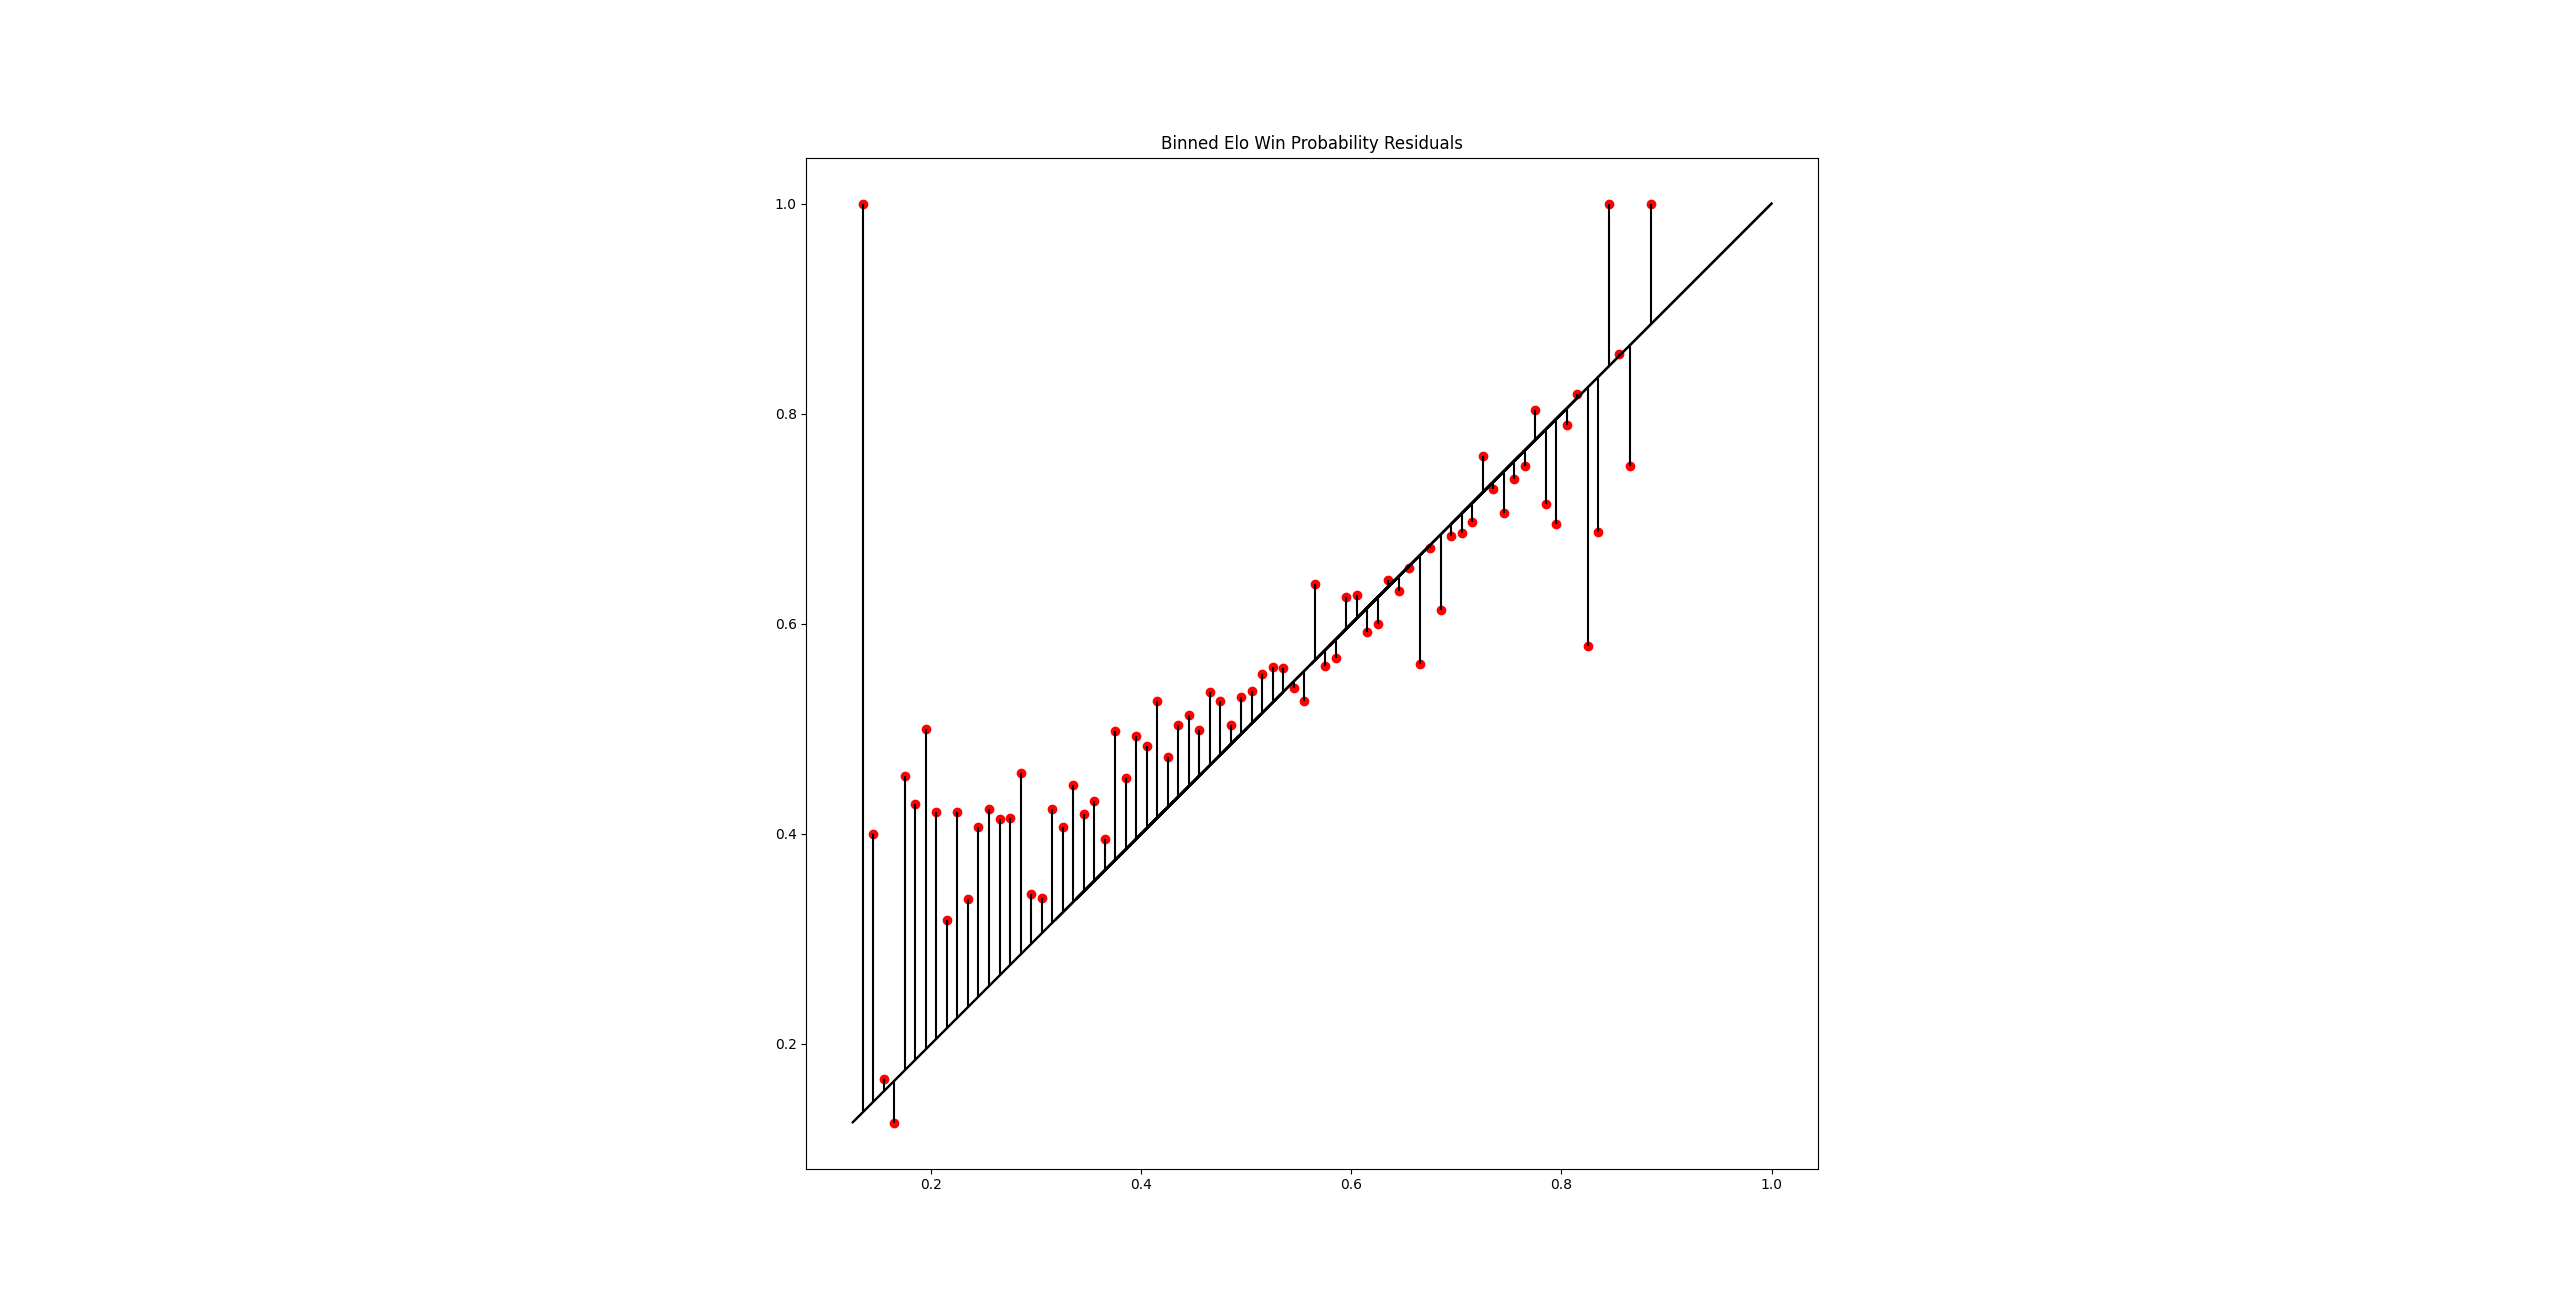
\includegraphics[width=2\textwidth]{elo_residuals.png}\\

\end{minipage}
  


\section{Related Work}
Similar work in this field has been done for other sports, such as the aforementioned ESPN Win Probability graph.
Some of the most useful work in this field has been done by groups studying Soccer like American Soccery Analysis using a 
machine learning based approach \cite{richardett} or research by Robberechts et al \cite{bayesian} using bayesian methods. Soccer
is a much more translatable sport to our problem, as it is also a low scoring game with a similar gameplay flow to hockey.
These works served as useful inspiration and insight into how we could develop an approach to predict the outcomes of hockey games.

\nocite{*}
\bibliographystyle{IEEEtran}
\bibliography{references}
\end{document}